\documentclass[11pt,letterpaper,oneside, titlepage]{scrartcl}
\usepackage{amsmath}
\usepackage{fancyhdr}
\usepackage{graphicx}

\usepackage[margin=1in]{geometry}


\pagestyle{fancy}
\fancyfoot{}
\fancyhead{}
\fancyfoot[CE,CO]{\thepage}
\fancyhead[LO,LE]{Detecting Texts Copied from a Common Source\\ Toth, Kiffer, Fein, Sheriff}

% disables chapter, section and subsection numbering
\setcounter{secnumdepth}{-1} 

\begin{document}
\title{Detecting Texts Copied from a Common Source}
\subtitle{CS 4780 Final Project Team 11}
\date{\today}
\author{Will Kiffer - wjk56\\Jeremy Fein - jdf226\\Kimberly Sheriff - kgs45\\Brian Toth - bdt25}
\maketitle


\tableofcontents
\clearpage

\section{Introduction}

The internet is filled with computer generated spam content meant to falsify search engine results, product reviews, and spam email detectors. Shady search engine optimization (SEO) companies flood websites with fake content in order to promote their customers. To create tremendous amounts of fake content that appears to be uniquely written, companies pay a human to write a single, unique article and then use techniques to transform, or “spin”, this article into millions of syntactically distinct but semantically identical articles. Although these articles may appear unique, they are actually inherently plagiarized. These millions of distinct articles are then posted automatically on blogs and review sites to promote or hyperlink to the SEO company's client. If web services could detect whether two pieces of content come from the same source, the reliability of aggregate measures online could be greatly improved.

In this paper we discuss novel methods of identifying whether two articles are generated from a common source. By exploiting the methodology of SEO companies, we aim to outperform simple methods such as cosine similarity. With a dataset of “article formulas” that can be used to generate millions of articles, learning can be done to predict if two articles are unique or plagiarized. Two methods, a discriminative analysis with SVM and generative modeling using HMM, are proposed, both of which perform better than simple cosine similarity. These methods could be deployed in a large scale spam detection service.

\section{Problem Definition and Methods}

\subsection{Task Definition}

Formally, our task is given a pair of articles A1 and A2, determine whether or not they are derived from a common source. Articles A1 and A2 are considered to be derived from a common source article B if both A1 and A2 are semantically identical to B. A1 and A2 are semantically identical if they can both be created by by algorithmically replacing words in B with contextual synonyms. These "synonyms" can be single words or groups of words. 

To accomplish this task we are using a manually processed database of articles obtained from a major SEO company. These articles are of the following form: ``I \{like\textbar love\} the \{small\textbar little\textbar medium-sized\} \{dogs\textbar canines\}''. A sample source article is included in Appendix A. From now on we will refer to a single group of contextually similar words/phrases such as \{really like\textbar love\textbar adore\} as a "spin group" and to individual members (really like, love, adore) as the spin group's members or elements. Note that not all phrases that make up a spin group need to have the same number of words. We will also refer to articles containing these spin groups as "source articles". An actual article can be generated by selecting one element from each spin group. SEO companies generate these source articles by paying a human to write a single article, using a computer to generate the spin groups, and then having a human postprocess the article to remove any spin group elements that would not grammatical or semantical sense. Appendix B shows two example generated articles from the source article in Appendix A.

Our dataset contains 2959 source articles. Each source article has on average 215.15 spin groups. Each spin group has on average 3.75 members. This means that each source article could potentially generate $3.18*10^{123}$ unique articles. These unique articles are correct both semantically and syntactically; they make sense. They are actual articles that you may find on the internet -- particularly on scam blog networks. They may not be the best written or most insightful articles, but they can easily be parsed by a native speaker.  However many of these "unique" articles are extremely similar. Some differ by one word, others only by a couple. However, even when they restrict themselves to the most dissimilar articles, SEO companies can still generate many articles.

The goal of this project is to create a similarity measure that, given two articles, will produce a number representing the articles' semantic similarity. This number can be used in a binary classifier to classify if the two articles are indeed from the same source or not. Using our dataset, we can generate numerous positive examples (two articles that are from a common source) and negative examples (two articles not from a common source), determine the similarity number for each example, and produce an ROC curve to show the effectiveness of our binary classifier. Our learned similarity measure should do better than a binary classifier using simple cosine similarity.

Each source article is also annotated with keywords describing each article. These keywords are useful for generating pairs of articles that are not duplicates, yet are still about the same topic. These pairs can be used as negative examples from our classifier. Without these keywords all our negative examples would be extremely dissimilar from the start just by virtue of being about different topics.

\subsection{Baseline}

The simplest baseline measure that we will use is cosine similarity between the two documents word vectors, where the word vectors are created using the bag of words model. Our classifier simply computes the cosine similarity between two documents and classifies them as duplicates if the similarity is above a certain threshold. We computed the cosine similarity for 1000 positive examples (pairs of duplicate articles) and 1000 negative examples (pairs of unique articles with the same keywords). We then computed the true positive rate and the false positive rate while varying the threshold value. Plotting these values we obtained the following ROC curve.

\begin{figure}[h!]
  \centering
  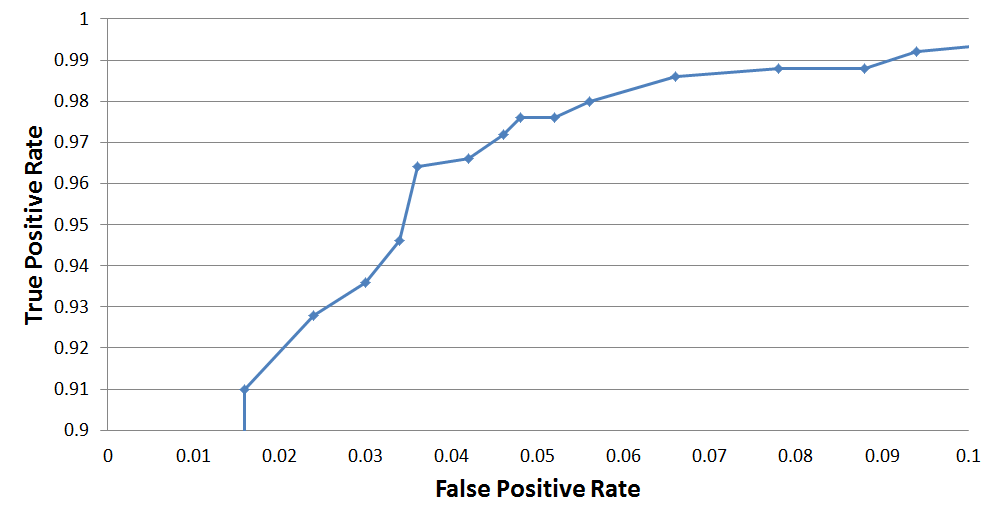
\includegraphics[width=1\textwidth]{baseline_ROC}
  \caption{Baseline ROC Curve}
  \label{fig:baseline_ROC}
\end{figure}

At it’s best, cosine similarity was able to achieve about a 96.5\% true positive rate and only about a 3.5\% false positive rate. Although this is already very good, the methods we describe below will be able to outperform these measures.


\subsection{Data Preprocessing}

Our data set of source articles is in .xml format. We parse the file into Python using the open source XMLToDict Python extension. Once in Python, it is simple to filter out blank or unusable source articles (those with bad formatting or limited keyword information) and provide ways to standardize the data. These standardizations include lemmatization of words, stemming of words, removing stop words, etc. Natural Language Toolkit (NLTK) and WordNet are used to achieve these tasks as shown in Figure ~\ref{fig:filtering}.

\begin{figure}[h!]
  \centering
  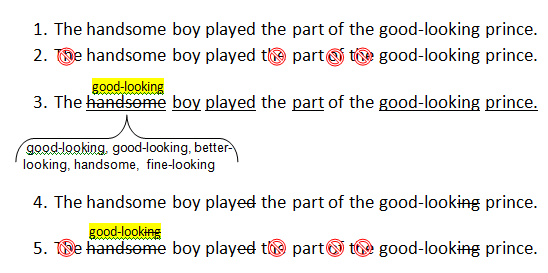
\includegraphics[width=0.75\textwidth]{filtering}
  \caption{Filtering Techniques}
  \label{fig:filtering}
\end{figure}

Figure~\ref{fig:filtering} shows a sample sentence (line 1) with the three techniques applied in isolation and together. Line 2 shows the effects of stop word removal. Line 3 shows synonym replacement where a word is replaced with its most common synonym. For example, if the words “like” “love” and “adore” all appeared in the data set, each instance of “like” “love” or “adore” would be replaced with “like.” In the example of line 2, NLTK and Wordnet were used to accomplish this task for each word in each article. First, the part of speech tagger in NLTK was used to denote the part of speech for the word "handsome", adjective.  Next, using the WordNet database, the synonyms for all senses of "handsome" the adjective were found and put into a list. Finally, this list of synonyms was sorted by order of frequency and the most common synonym replaced the word. Line 4 shows the stemming of words. In this case, "played" becomes "play". Line 5 shows the combination of all three techniques with stemming occurring last.

In addition to filtering individual articles, we can also determine the types of articles to be used in our training and test sets. Since each article is denoted by a set of keywords, we can choose to use only articles that share every keyword, at least one keyword, or give no restrictions on keyword similarity.

To ensure that we are using similar training and test sets for all methods, we decided to train and validate on odd numbered source articles and test on even numbered source articles.

\subsection{SVM Approach}

This supervised learning approach uses a soft margin support vector machine (SVM) to classify articles. Each spun article is labeled with the number of the source article that it comes from. We generate a binary classifier for each source article and then use a 1-vs-all method to classify each article into the source that it matches most closely. This method has the potential to be very useful because it does not require specific knowledge about the form of the source articles; only knowledge of the source article that each spun article came from.

We hypothesize that, given two articles A1 and A2, this model can be used to determine if A1 and A2 came from the same article by running both articles through each classifier. If the two articles come from the same source, they should both be classified as coming from that source with a reasonable degree of confidence.

\subsection{HMM Approach}

Our generative approach aims to use a hidden markov model (HMM) to predict a hidden source article that could have generated an actual article. The intuition is that a sentence in an actual article can be modeled as a sequence of phrases that was emitted from a hidden sequence of spin groups. Each spin group in our known source articles can be modeled as a hidden state; a single hidden spin group state has equal chance to emit any of its elements. Transitions between hidden spin group states are drawn from the sequences of spin groups in the known source articles. With these transition and emission probabilities, a modified Viterbi algorithm can predict a sequence of spin groups from an article. We hypothesize that this sequence of spin groups is essentially the result of adding in possible contextual synonyms to the article -- just as is done when a human writes a source article.

Moving forward with this approach, a primary initial concern is the running time of the Viterbi algorithm. Many of our decisions will be motivated by the desire to keep the running time as low as possible, which is mainly influenced by the number of hidden states (number of unique spin groups).

We hypothesize that, given two articles A1 and A2, this generative model can be used on A1 to predict a potential source article S1 that is semantically likely to have generated A1. Then, if A1 and A2 were actually from a common source, S1 would also be able to semantically generate A2.


\section{Experimental and Theoretical Evaluation }

\subsection{SVM Methodology}

%What are the criteria you are using to evaluate? How does this evaluation (e.g. experiment) relate to the questions you are trying to answer? Describe the experimental methodology that you used. What is the training/test data that was used, and why is it realistic or interesting? Exactly what performance data did you collect and how are you presenting and analyzing it? Comparisons to competing methods that address the same problem or to variations of your own algorithm are particularly useful. Give enough detail about your experiment setup so that others could reproduce the work.
%TODO
%<SVM METHODOLOGY AND EVALUATION CRITERIA HERE>

First, spun articles were generated and paired to create positive (from the same source article) and negative (from different source articles) examples.  Then one of the filtering methods was applied.  The resulting data was split into test, training, and validation sets.  The test set contained 30\% of the examples and the rest of the examples were used for training and validation. Each training set contained 56\% of the examples, and each validation set contained 14\% of the examples.

The classifier for each source article was generated by relabeling the spun articles as +1 if the article came from the current source or -1 if the article did not come from that source. The feature vector for each article was a simple bag of words. These labels and feature vectors were fed into SVMlite. Five fold cross validation was used to maximize average accuracy on the validation sets. C values were chosen from the range [0.001, 0.01, 0.1, 1, 5, 10]. Ultimately, accuracy was measured against the test set to produce the results below.

\subsection{SVM Results}

%Present the quantitative results of your experiments. Graphical data presentation such as graphs and histograms are frequently better than tables. Explain the basic findings by explaining the results contained in the tables and graphs.

The results showed that filtering does improve accuracy in learning as shown in Figure~\ref{fig:svm}. The baseline gives the SVM method an accuracy of 66\%, but nearly 100\% when all filtering methods are used. The filtering techniques in rough order of efficacy are: stopwords removed, replaced synonyms, and standardized articles. Standardized articles refers to stemming and lemmatizing the articles.


\begin{figure}[h!]
  \centering
  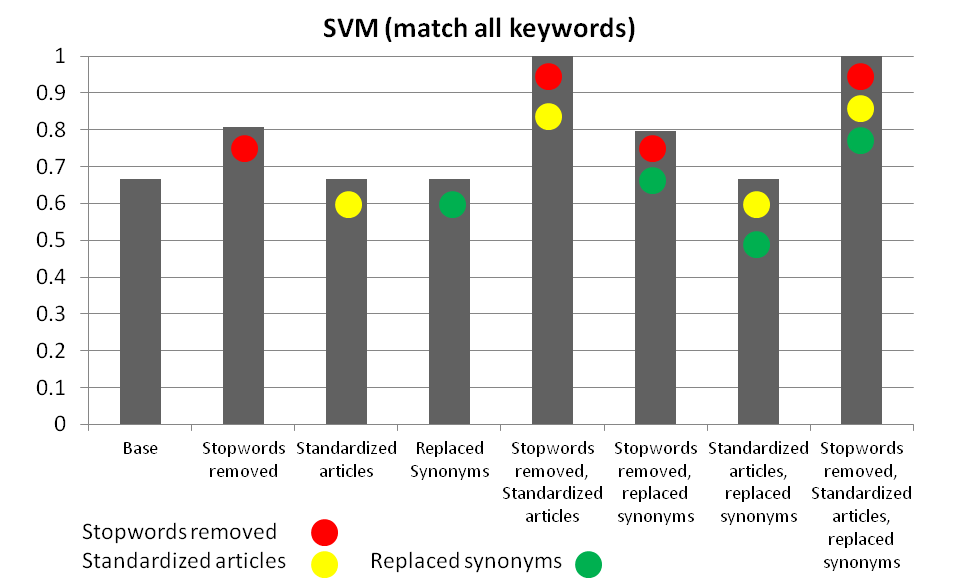
\includegraphics[width=0.75\textwidth]{svm_allmatches}
  \caption{SVM Results Histogram}
  \label{fig:svm}
\end{figure}

\subsection{HMM Methodology}

To create a working HMM model, we first need to model all source articles as sequences of spin groups. Words in source articles that are not members of spin groups are treated as a spin group with one element of that word. For example “I {like\textbar love} the {dog\textbar canine},” transforms into the spin groups “{I}, {like\textbar love}, {the}, {dog\textbar canine}”.

Our HMM is designed to classify a single sentence. Therefore to classify an article, we classify each sentence individually. We chose to classify sentences at a time for two reasons. First, transitioning between the last spin group of a sentence and the first spin group of the next sentence doesn’t make much sense. Intuitively, the word that starts a sentence has little to do with the word that ended the last sentence. Additionally, if our HMM classified articles as a whole, the start probabilities would be which spin groups are most likely to start an article. Again, this seems to make less sense than the alternative of classifying a single sentence, where the start probabilities would be which spin groups are most likely to start a sentence. Finally, it would be easy for a computer to add more variability to generated spam articles by switching sentence order; by treating each sentence individually, this trick should not matter in our final classification.

\subsubsection{Clustering}

Our dataset contains over 150,000 unique spin groups. Running Viterbi on this large of a state space is simply unfeasible, so we need to reduce the number of spin groups. The most obvious way to reduce the number of spin groups is to use spin groups seen in a random subset of the source articles. While this approach is effective at reducing the number of spin groups and is easy to implement, it is not ideal since we lose information by just taking a random subset.

A better approach is to use a clustering method to reduce the number of spin group states. This has the added benefit of smoothing some of the noise in the dataset, where unique spin groups only differ by a single word. However, we have to be very careful when we attempt this clustering so that we don’t accidentally combine two spin groups that are actually semantically different and therefore lose information.

Because of this, we chose to use HAC clustering with complete-link similarity. Similarity between two spin groups was computed as the number of elements the spin groups have in common divided by the total number of elements in both spin groups. Complete-link was used to ensure that all members of a cluster were similar to every other member.

However even clustering was infeasible on 150,000 spin groups. We therefore only used spin groups from 250 random training articles which turned out to be around 25,000. We then clustered these spin groups into about 13,000 spin group clusters. These spin group clusters are the hidden states.

\subsubsection{Transition probability estimation}

Although we were only able to use spin groups gathered from 250 training articles, we could use the entire training set to estimate transition probabilities between spin group clusters. To do this, we keep track of the set of unique spin groups as well as a mapping from each spin group to the cluster of spin groups that it belongs to. Then, for each sentence in each source article in our training set, we look at every bigram of spin groups. We map the spin groups in the bigram to clusters, and keep track of the number of times a unique cluster occurs in our training set. If both spin groups map to clusters (meaning we have seen both spin groups in the original 250 random training articles the spin group clusters were derived from), then we increase the number of times the first spin group cluster can transition to the second spin group cluster. Using these bigram counts, we can calculate the transition probability between two spin group clusters.

Since we have not seen every possible bigram in our training data, many unseen bigrams will have a 0\% probability of occurring. To fix this, we introduce Witten-Bell smoothing, where the probability of an unseen bigram occurring will be estimated by the unigram probabilities of the spin group clusters and the number of times those spin groups are involved in bigrams in general. This allows our HMM to sometimes predict untrained transitions that may ultimately lead to a more semantic spin group prediction.

\subsubsection{Emission probability estimation}

The probability that a given spin group cluster will emit a given phrase is the chance that, if an element were to be picked at random from the spin group cluster, it will be the given phrase. If the phrase is part of the spin group cluster, this will be exactly 1 divided by the number of elements in the spin group. If not, then this is exactly 0.

\subsubsection{Modified Viterbi}

Our implementation of Viterbi was straightforward except for one part. Since spin group elements could be variable length (such as ``\{like\textbar really like\}”) this meant that one hidden spin group state could potentially generate more than one output state. To do this, we modified Viterbi so that a state was a tuple of (Spin group, Number of output states it generated). From analyzing our dataset, we found that over 99\% of spin groups had no elements longer than 4 words. We therefore allowed the number of output states a spin group generated vary from 1-4, and effectively quadrupled our state space. 

We also created an additional special hidden state for unknown words. If we have never encountered a word before, then the emission probability for every state will be 0, and therefore we just assign it to the unknown state. Below is a diagram illustrating how this modified Viterbi algorithm worked.

\begin{figure}[h!]
  \centering
  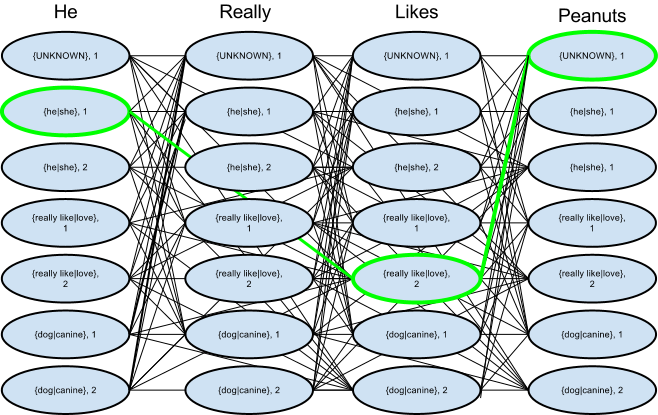
\includegraphics[width=.8\textwidth]{hmm_spin_group}
  \caption{HMM Spin Group}
  \label{fig:hmm_spin_group}
\end{figure}


In the above example the hidden spin group \{really like\textbar love\} generated the two output states ``really like", and since we have never seen the word ``peanut" before, it is assigned the unknown spin group.

\subsubsection{Evaluation}

With a working HMM model to predict the most likely sequence of spin groups that could have generated a given article, we can then experimentally test our hypothesis stated. Again, our hypothesis is that given articles A1 and A2, we can make spin group predictions S1 and S2; if potential common source S1 is equally likely to generate A1 and A2, and other potential common source S2 is equally likely to generate A2 and A1, then it is likely A1 and A2 are from the same common source. Since some words in A2 will not be present in S1, there would be a 0\% chance that S1 would emit A2; thus, we need a better measure to show if S1 (or S2) could equally generate A1 and A2. Instead, it is thought that if S1 can generate A1 and A2 equally, then the cosine similarity between S1 and A1 should be similar to the cosine similarity between S1 and A2. The ratio of these cosine similarities would tell us how similar they are -- if the similarities are the same, the ratio will be 1, and if they are disparate it will be less than 1 (A2 will never be more similar than A1). Cosine similarity is done on word count vectors of the words in spin groups and in the articles. We can then average the cosine similarity ratios for S1 and S2 to produce an overall similarity measure for A1 and A2:

$Similarity(A1, A2) = AVG\{ cos(A2, S1)cos(A1, S1) , cos(A1, S2)cos(A2, S2) \}$

This measure can then be placed in a binary classifier with varying thresholds to make an ROC graph to rate the effectiveness of the similarity measure in a binary classifier. The HMM is trained on even numbered source articles, and positive/negative examples are drawn from only odd numbered source articles. Remember, negative examples (two articles not from a common source) are chosen to have the same keywords and thus be about the same topic.

\subsection{HMM Results}

\begin{figure}[h!]
  \centering
  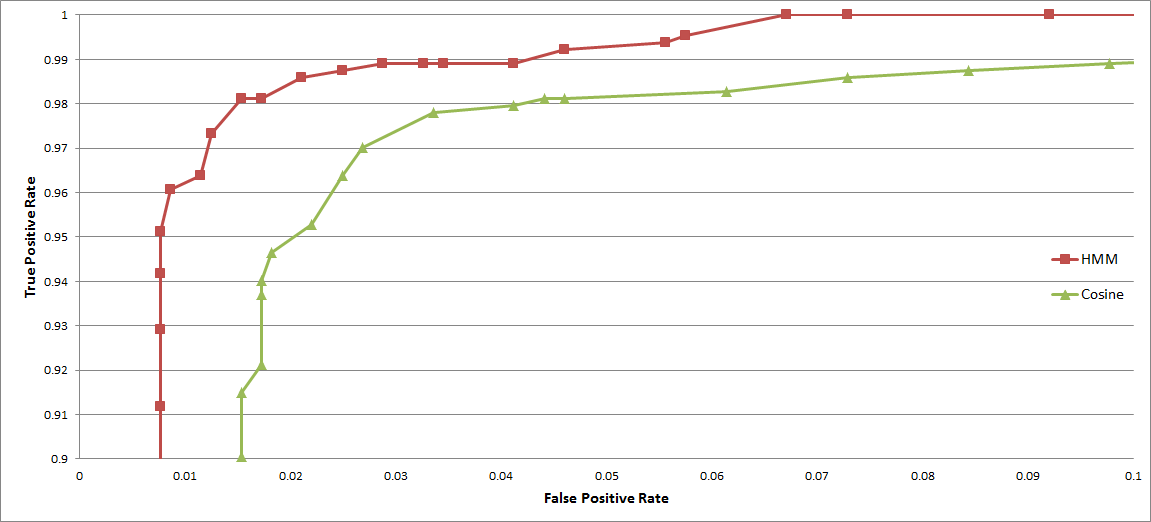
\includegraphics[width=1\textwidth]{hmm_ROC}
  \caption{HMM ROC Curve}
  \label{fig:hmm_ROC}
\end{figure}

The above ROC graph shows results for running our HMM classification in a binary classifier on 634 total positive and 1043 total negative examples. A positive example consisted of two articles generated from the same source article and their HMM spin group classifications. A negative example consisted of two articles generated from different source articles (with the same keywords) and their HMM spin group classifications. All of these examples were drawn from odd numbered source articles, and the HMM was trained on only even numbered source articles. Because of the long running time of HMM, we could not classify both articles in all examples in our original testing set. Instead, we classified these 1677 data points chosen at randomly from our original test set. Generating an ROC graph with cosine similarity on these 1677 data points yields similar results as our baseline ROC; thus, we are confident that this small data set should appropriately show the effectiveness of our HMM-based similarity measure.

At best, our HMM-based binary classifier achieves a 98\% true positive rate and 1.5\% false positive rate. This compares well against 96\% true positive rate and 2.5\% false positive rate for cosine similarity on the same data. Thus, our classification scheme is able to better discriminate if two articles are similar with a greater range of variability in the articles; it can better capture articles that have lots of words in common but are different and vis versa. Since we use cosine analysis to compare the HMM classifications, performing an HMM classification of an article is essentially adding into the article more contextual synonyms. Thus, these synonyms must be in the other article as well, and we appropriately capture this to say if the articles are similar or not.


\subsection{Discussion}

Our HMM implementation performs extremely well, even better than cosine similarity. Intuitively, the HMM takes an article, and attempts to replace words and phrases in the article with groups of contextual synonyms. By doing this, we are essentially doing what an SEO company does when they pay a human to write a single article, use a computer program to generate the source article containing spin groups, and finally have the human prune the source article to remove synonyms that are grammatically or semantically incorrect. While current methods exist to replace words and phrases with groups of synonyms, the true value of our HMM lies in the transition probabilities between spin groups. By using these transition probabilities, our HMM in theory should only replace words or phrases with groups of synonyms which make sense both grammatically and semantically (in essence doing the work of the human who prunes the source articles). 

These results also demonstrate that this approach generalizes well to articles about topics that the HMM was not trained on. This is because even if our HMM has never seen articles about a certain topic, it will still have seen many of the words or phrases in the article. In addition, when it comes to the types of articles that SEO companies generate, unknown words are very likely to not be part of a spin group, and therefore not be different between duplicate articles. The reason for this is if an SEO company were promoting a site about suits, it would want the word suits to appear in the article as often as possible, and therefore would not replace it with any other synonym. Our HMM therefore handles these unknown words correctly by not replacing them with a spin group. 

However, we cannot say with total certainty that this approach would generalize well to articles plagiarized using more advanced techniques rather than just replacing words and phrases with groups of contextual synonyms. This would be an interesting question for follow up work. One thing that is clear is that since our HMM classifies sentences at a time rather than entire articles, it would not be fooled by simply rearranging sentences. However, since SEO companies are mostly concerned with maximizing the number of articles they can generate for the lowest cost, it is reasonable to believe that the majority of SEO generated spam is generated using methods similar to source articles we trained our HMM on.

Lastly, although running time was a major problem for us, it does not rule HMM out for actual use in industry. Our method could be parallelized extremely easily. Each sentence could be classified by a single machine, and therefore an article could be classified in a very short amount of time. Additionally this method could be used as a supplement to cosine similarity rather than a replacement. Companies could choose to only run HMM on articles that have a cosine similarity above a certain threshold.

Although the SVM method performs well when combined with filtering, its superiority to cosine similarity (when also combined with the same filtering) is not statistically significant.  We believe that this is a result of many common words existing in all articles spun from the same source.

\section{Related Work}

%Can you say anything about related work from your background readings? It may be possible to answer the following questions for each piece of related work that addresses the same or a similar problem. What is their problem and method? How is your problem and method different? Why is your problem and method better? 

Fingerprinting is the current most commonly used method of plagiarism detection. This method creates a representation of a document by creating a set of n-gram phrases. The sets are referred to as the fingerprints and the phrases are called minutiae. The minutiae are checked against a known reference set to determine if the document is plagiarized or not. The number of n-grams is determined by the importance of the plagiarism detection and the time constraint. This method is not effective for data sets like ours in which words my be replaced with a single synonym or with a group of words which have the same meaning.

\section{Future Work}
The SVM method could be improved by introducing more filtering along the same lines as the existing filters and further exploring thresholding.  Thresholding is the use of an artificial minimum similarity; if an article falls below this threshold for every source article it is classified as unique.  For our work we used a low, fixed value that produced good results as the threshold, but this number could be determined experimentally.  In addition, an alternative SVM implementation could attempt to learn the characteristics common to most spun articles (the words frequently used in source articles).  Positive examples would be spun articles from all source articles, and negative examples would be real articles about similar topics from sources such as Wikipedia.

For HMM, one of the main limitations is the sheer amount of time that classifying a single article requires. As a result, we were only able to use a fraction of the spin groups that were present in our training set. In the future, clustering could be used even more to raise the number of spin groups we were able to utilize. K-means clustering could be used to target a specific number of clusters that would result in Viterbi running in a reasonable amount of time. However targeting too few clusters may lead to dissimilar spin groups being clustered together, which may affect the accuracy of our HMM method.

Also, currently when we estimate transition probabilities, if we have not seen one of the spin groups in a spin group bigram, then we just ignore the bigram. However, we are essentially losing information when we do this. Instead we could keep track of the unigram probabilities for all spin groups, even ones that we have not seen before. We could then use these unigram probabilities for a more accurate smoothing algorithm. Additionally, an unseen spin group could be matched to the most similar seen spin group, and if the similarity is high enough we could just treat it as it were the seen spin, essentially clustering as we go along. However this method may increase the running time of training step by a huge amount if we need to compare every unseen spin group to every seen spin group.
 
%TODO What are the major shortcomings of your current method? For each shortcoming, propose additions or enhancements that would help overcome it.

\section{Conclusion}

We explored two very different methods of identifying computer-generated content and achieved considerable success with both.  Using a discriminative method involving SVMs and filtering, we achieved nearly 100\% accuracy modeling the spun articles as simple bags of words.  Even better was the generative method using HMMs which performed strictly better than our baseline cosine similarity measure.

\section{References}

Hoad, Timothy C., and Justin Zobel. "Methods for Identifying Versioned and Plagiarized Documents." Journal of the American Society for Information Science and Technology 54.3 (2003): 203-15. Print.

\section{Appendices}

\subsection{Appendix A: Snippet of Sample Source Article}

\begin{verbatim}{Whenever|When|At any time when|When you are|Whenever you are|Should you be|If you're|
If you happen to be|If in case you're} {planning|preparing|organizing|setting up} 
{weddings|wedding ceremonies|marriage ceremonies|wedding events}, the groom {and the|
and also the|plus the} {bride|bride-to-be|new bride} {need to|have to|really need to|
will need to} {think about|consider|take into consideration|contemplate} {everything|
every thing|almost everything} {in order to|as a way to|so that you can|to be able to}
{please|satisfy|gratify|entertain} {all the|all of the|every one of the|each of the}
{people|individuals|men and women} {attending|visiting}. {One of the|Among the|
One of several|One of the several} {problems|issues|troubles|complications} that 
{usually|generally|typically|commonly} {appears|shows up|arises|comes up} is what 
{souvenirs|mementos|gifts} to be {used|utilized|employed}. {Most of them|Many of them|
A lot of them|Some of them} are {designed|created|developed|made} for female {guests|
visitors|attendees} {and not|rather than|instead of} for the men. {Because|
Simply because|Due to the fact} of this, it {might|may|could} be a {great|fantastic|
good} {idea|concept|notion|strategy|plan} {to use|to make use of|to implement} koozies
for wedding favors, {as they|because they|since they} are {perfect|ideal|best} for 
{male|men|guys} {guests|visitors|attendees}.
\end{verbatim}
 
\subsection{Appendix B: Two Resulting spun article from Appendix A}


Should you be preparing weddings, the groom and the bridetobe will need to think about everything in order to satisfy all of the individuals attending. One of several issues that commonly appears is what gifts to be employed. Many of them are created for female attendees instead of for the men. Simply because of this, it might be a fantastic idea to use koozies for wedding favors since they are perfect for male attendees.
\\

Whenever organizing wedding events, the groom and also the bride have to take into consideration almost everything as a way to please every one of the people visiting. One of the several problems that usually shows up is what souvenirs to be used. Some of them are made for female visitors and not for the men. Because of this, it could be a great concept to implement koozies for wedding favors, because they are ideal for guys visitors.

\end{document}
